%!TEX root = bachelor.tex
\chapter{Analyse}
\label{ch:analysis}
\todo{analyse einleitung schreiben}
In diesem Kapitel...

Zunächst werden die beiden Verfahren zur Entzerrung gegenübergestellt. Anschließend untersuchen wir verschiedene Einflüsse auf der Qualität der Entzerrung, woraufhin wir die Laufzeit ermitteln. 
Zum Schluss Ransac...

Die Laufzeitanalysen wurden auf einem Raspberry Pi 2 Model B durchgeführt mit folgenden Eigenschaften:
\begin{itemize}
	\item 900MHz ARM Cortex-A7 CPU
	\item 1GB RAM
	\item GCC-4.9.2
	\item Opencv 2.4.13
\end{itemize}


\section{Vergleich Vorwärtsentfaltung und Rückwärtsentfaltung}
In Kapitel \ref{ch:method} haben wir festgestellt, dass das entfaltete Bild mittels Vorwärtsentfaltung Löcher enthält. Es ist hierbei von Interesse wie sich die Anzahl der Löcher bei einer Änderung der Auflösung verhält. Der Einfluss der Ausgabeauflösung auf die Anzahl der Löcher lässt sich in Abbildung \ref{fig:influenceRes} ablesen. 

\begin{figure}[!htb]
	\centering
	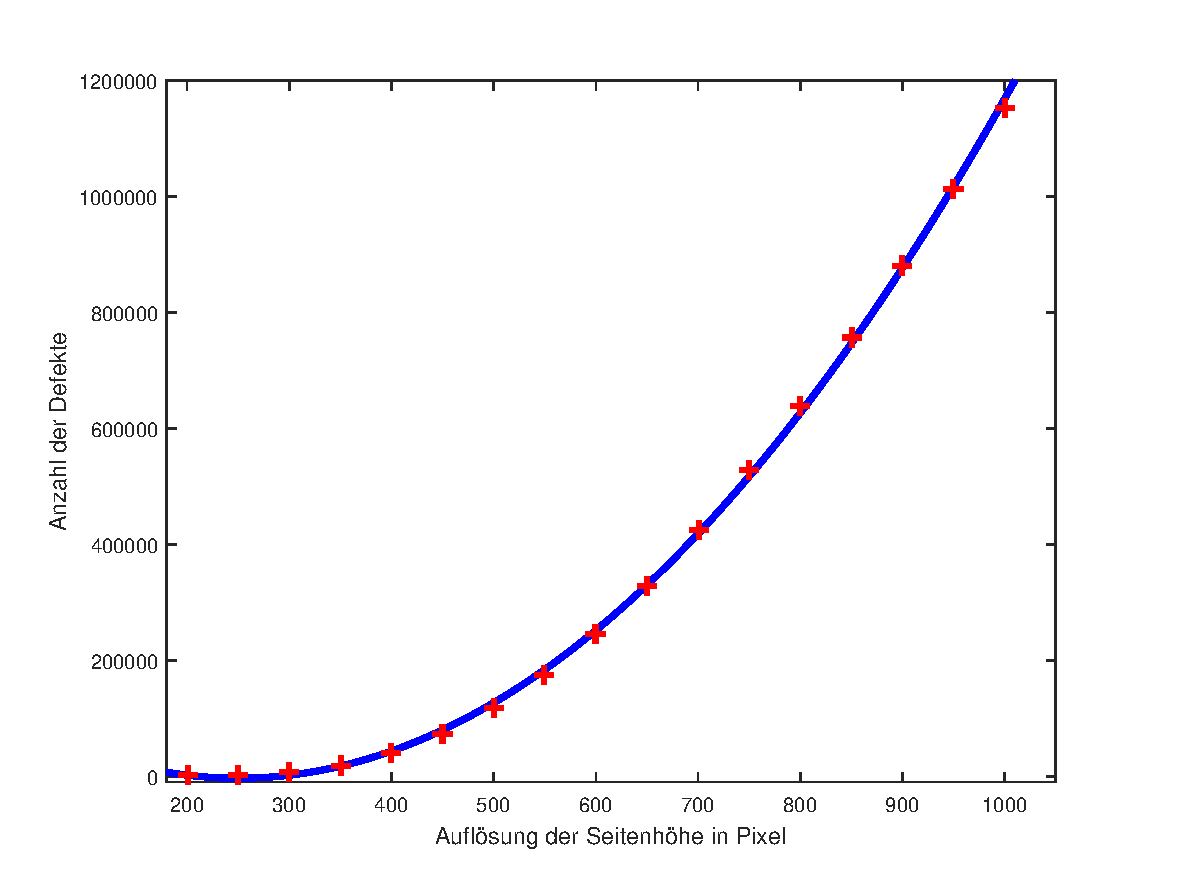
\includegraphics[width=\textwidth]{images/numberOfHoles.eps}
	\caption{Einfluss der Ausgabeauflösung auf die Anzahl der Löcher}
	\label{fig:influenceRes}
\end{figure}

Wie erwartet verhält sich die Anzahl der Löcher quadratisch zur gewählten Ausgabeaufösung. Der Informationsgehalt (Pixelanzahl) des Ursprungsbild bleibt natürlich trotz erhöhter Ausgabeauflösung konstant. Da sich die Auflösung der Seitenhöhe quadratisch zur Gesamtanzahl der Pixel verhält, ist auch ein quadratisches Wachstum der Anzahl der Löcher zu erwarten. 
\bigskip

Als Reprojektionsfehler einer Abbildung wird die Distanz zwischen einem gemessenem Punkt und einem korrespondierendem projizierten Punkt bezeichnet. 
\bigskip

Im Falle der Rückwärtsentfaltung sind die gemessenen Punkte die Bildpositionen der Samples im Ursprungsbild. Da die Geometrie des Kegels bekannt ist, wissen wir wo sich die  Samples auf dem entfalteten Bild befinden müssen (siehe Parametrisierung der Mantelfläche \ref{eq:paramLateral} in Kapitel \ref{ch:theory}). Wir können nun diese Positionen mit Hilfe der Abbildung zur Entfaltung und der Projektionsmatrix zurück auf das Ursprungsbild abbilden. Diese Punkte sind die projizierten Punkte. Da die Abbildung von der Mantelfläche zur Kegeloberfläche exakt ist, ist der Reprojektionsfehler der Rückwärtsentfaltung alleine durch die Projektionsmatrix bestimmt. 

Bei der Vorwärtsentfaltung sind die gemessenen Punkte gegeben durch die bekannten Sample-Positionen auf der Mantelfläche. Die Projizierten erhält man, nach der Abbildung der detektierten Sample-Positionen des Ursprungsbild auf die Mantelfläche. Der Reprojektionsfehler ist also alleine durch die Genaugkeit der Sample-Detektion definiert und somit bei diesem Verfahren immer nahe null. 
Obwohl das Endergebnis, bedingt durch die Löcher, bei der Vorwärtsentfaltung optisch schlechter ist, ist der Reprojektionsfehler also bei der Vorwärtsentfaltung immer kleiner. 
Als Vergleich zwischen den beiden Verfahren eignet sich der Reprojektionsfehler also nicht.

\begin{figure}[!htb]
	\centering
	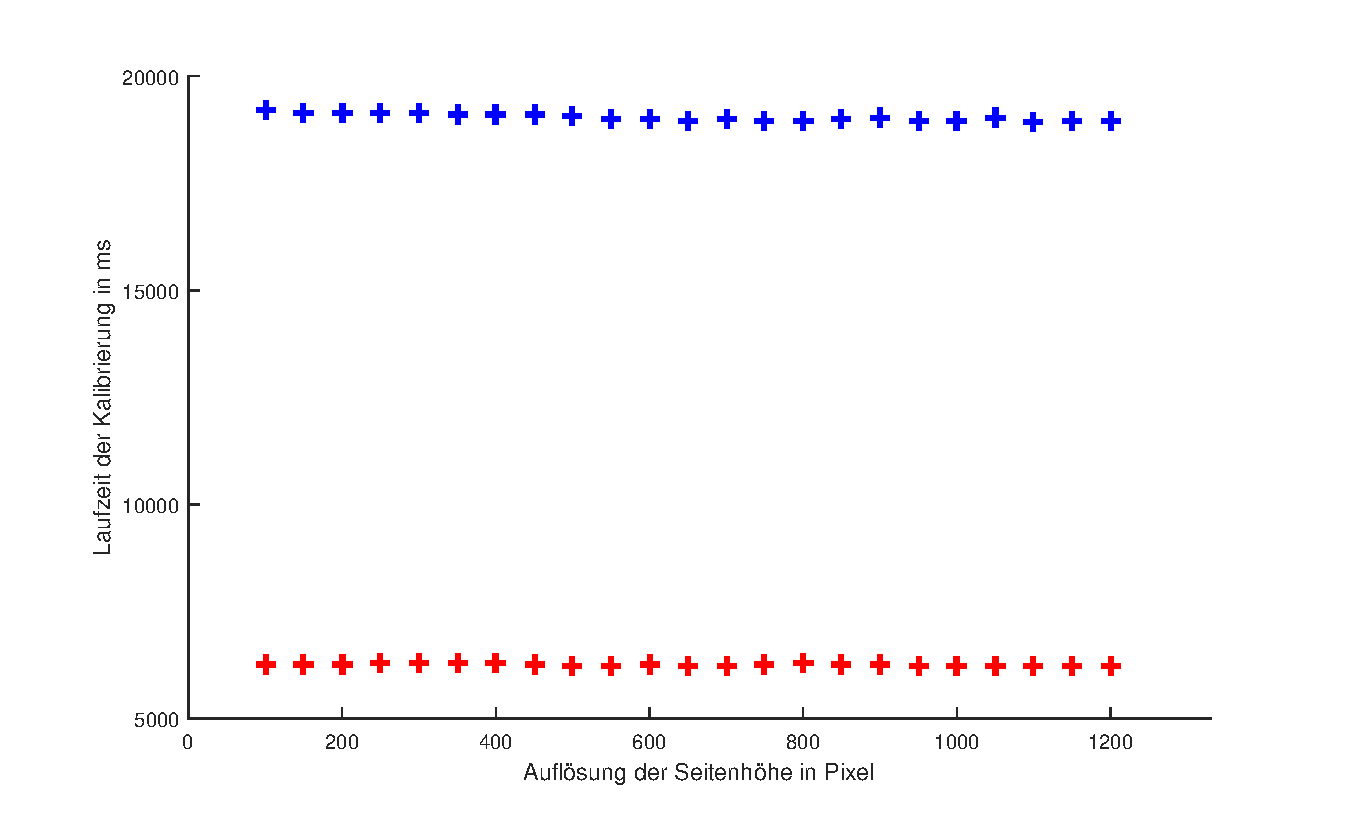
\includegraphics[width=\textwidth]{images/runningTimeCalibration.eps}
	\caption{Laufzeitvergleich zwischen Vorwärtsentfaltung (blau) und Rückwärtsentfaltung (rot)}
	\label{fig:runningTimeComparision}
\end{figure}

Wir entscheiden uns optisch und auf Grund der schlechteren Laufzeit bei der Vorwärtsentfaltung (siehe Abbildung \ref{fig:runningTimeComparision}) für die Rückwärtsentfaltung. 
Alle weiteren Auswertungen beziehen sich von nun an auf die Rückwärtsentfaltung.

\section{Einfluss der intrinsischen Kalibrierung}
Ein wichtiger Einflussfaktor auf die Qualität der Entfaltung ist die intrinsische Kamerakalibrierung, die vor der eigentlichen Kegelkalibrierung stattfindet. Ihre Hauptaufgabe besteht darin, die Linsenverzerrungen der Kamera herauszurechnen. 

Wir messen den Einfluss der Kamerakalibrierung mit Hilfe des Reprojektionsfehlers. Dazu betrachten wir fünf verschiedene Bilder, die ein Mal mit und ein Mal ohne intrinsische Kalibrierung entzerrt werden. Bei beiden Gruppen wird anschließend jeweils der Reprojektionsfehler pro Sample bestimmt und verglichen. Die Ergebnisse sind in Abbildung \ref{fig:influenceCalib} zu sehen. In der linken Abbildung sind hierbei die Fehler im kalibrierten Fall zu erkennen, im Linken im Unkalibrierten. In der Abbildung ist dabei ein Kreuz bei $(u,v)$, falls die Abweichung des projizierten Punktes in $x$-Richtung $u$, sowie in $y$-Richtung $v$ beträgt. 

\begin{figure}[!htb]
	\centering
	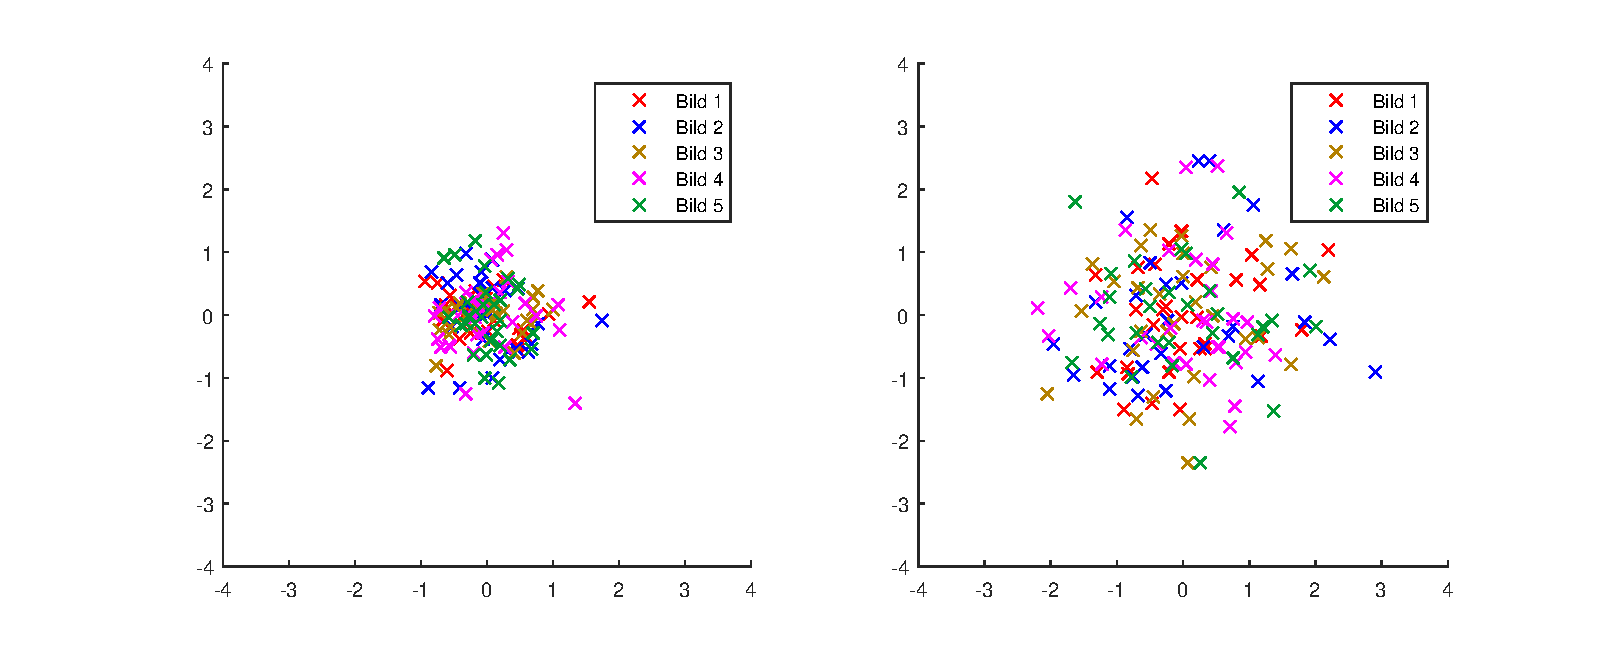
\includegraphics[width=\textwidth]{images/reprojectionErrorReverse.eps}
	\caption{Einfluss der intrinsischen Kalibrierung auf den Reprojektionsfehler}
	\label{fig:influenceCalib}
\end{figure}


Es ist klar zu erkennen, dass die Reprojektionsfehler bei den Bildern ohne intrinsische Kamerakalibrierung wesentlich größer ist. Der starke Einfluss kommt unter Anderem daher, dass wir eine Weitwinkelkamera mit starker tonnenförmiger Verzerrung eingesetzt haben. Ohne eine Modellierung der Linsenverzerrungen weichen die Abstände zwischen den Sample-Positionen stark von der Realität ab. Die Projektionsmatrix wird mit fehlerhaften Daten bestimmt. 

\section{Einfluss der Rotation der Kamera}
Um den Einfluss der Rotation der Kamera untersuchen zu können, wurde der Kegel mit Kalibrierungsmuster gerendert, da die Kameraposition dann exakt bekannt ist und äußere Faktoren wie Lichtverhältnisse und inhomogene Hintergründe kontrolliert werden können. 

\begin{figure}[!htb]
	\centering
	\begin{subfigure}{.5\textwidth}
		\centering
		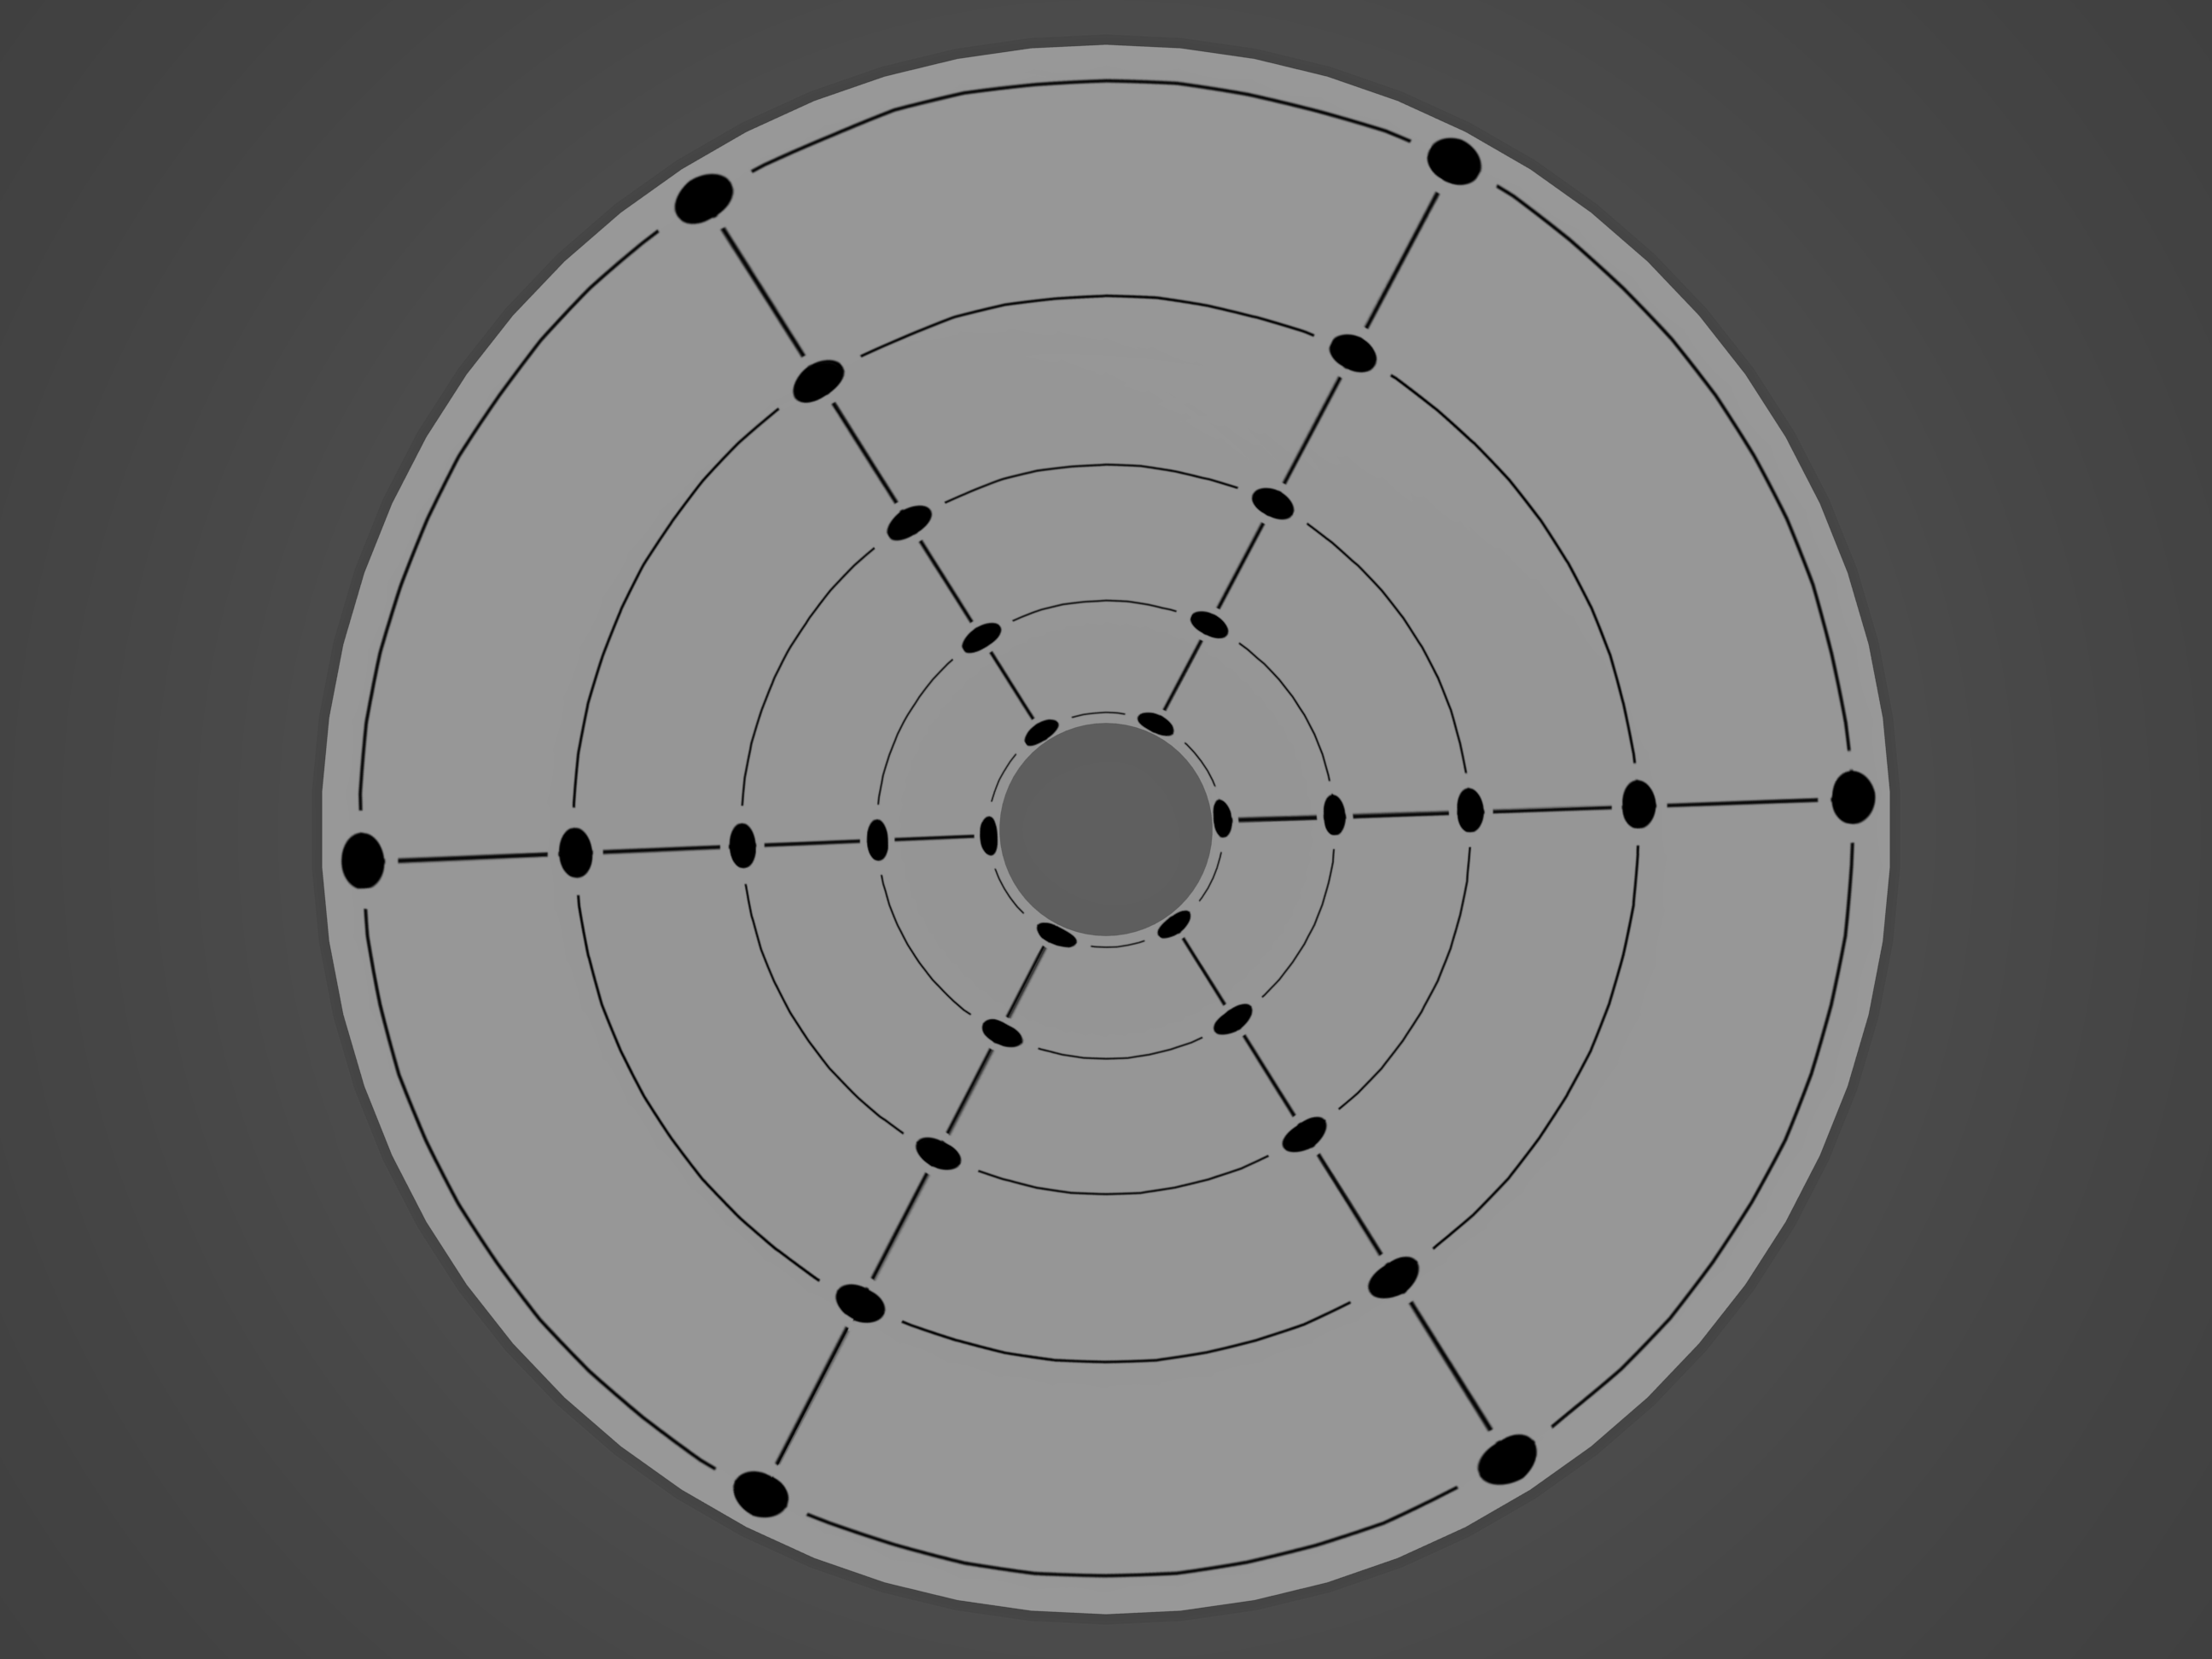
\includegraphics[width=.9\textwidth]{images/blender0.png}
		\caption{bei 0°}
	\end{subfigure}%
	\begin{subfigure}{.5\textwidth}
		\centering
		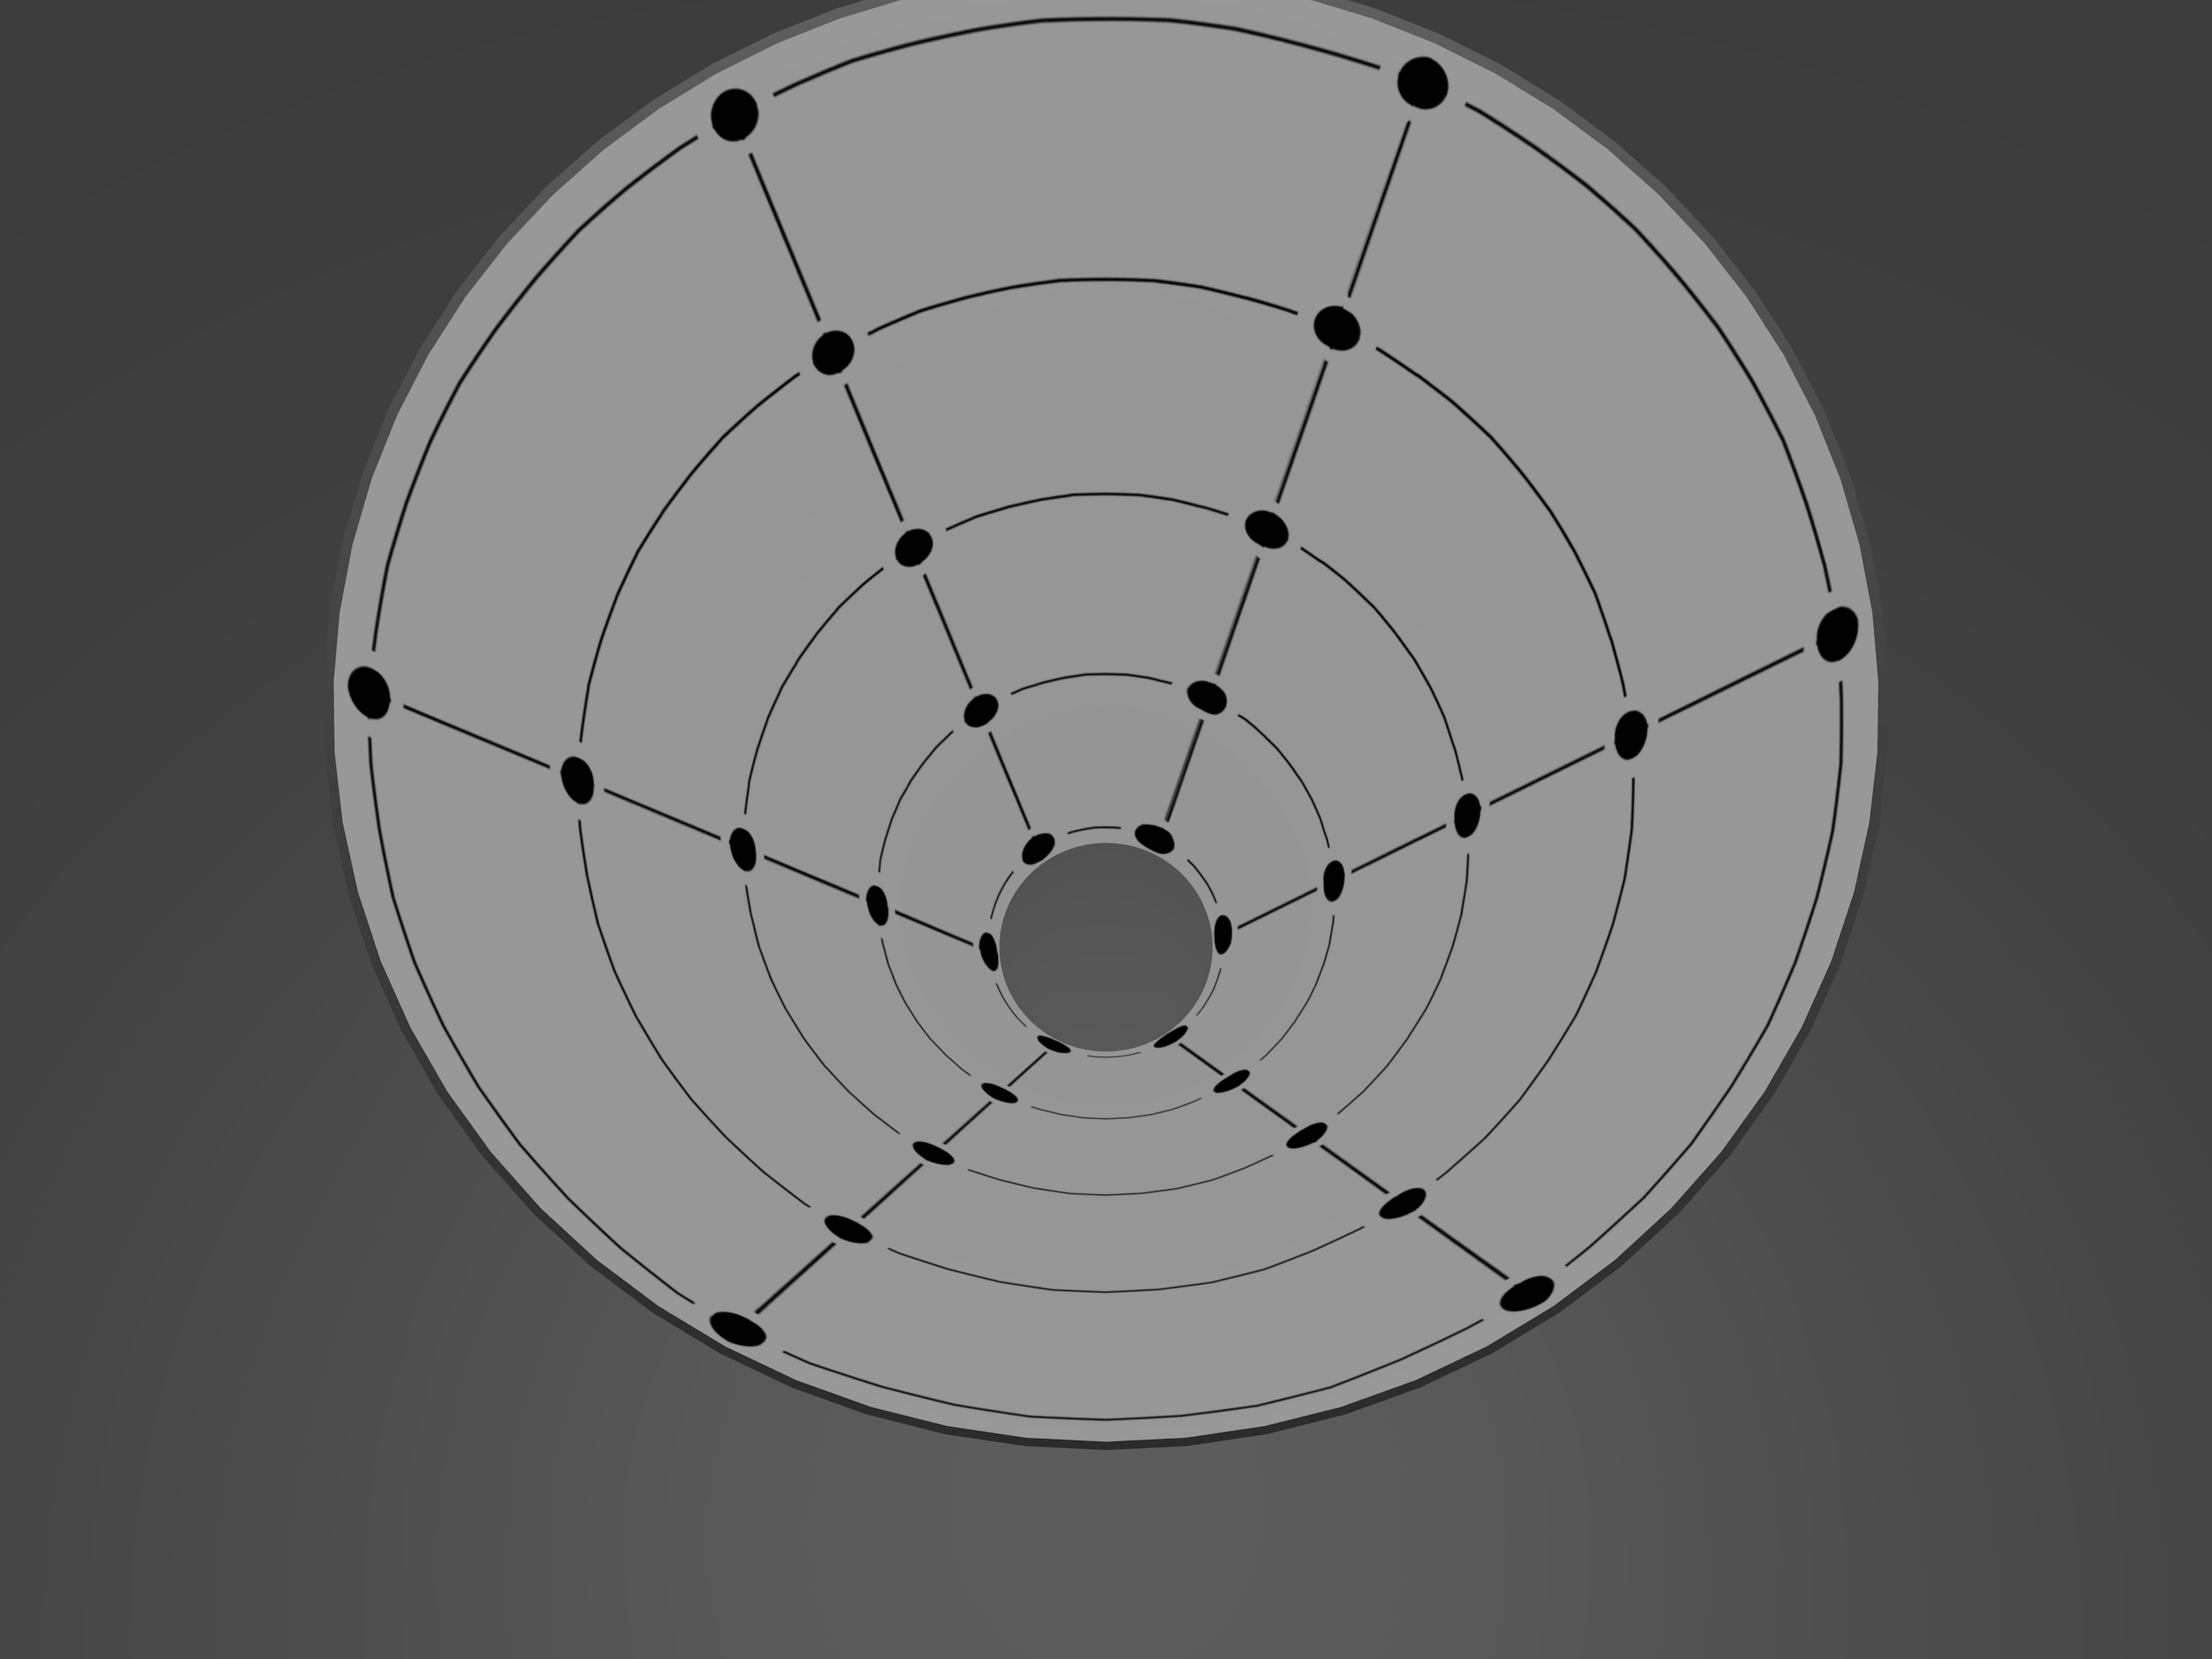
\includegraphics[width=.9\textwidth]{images/blender12.png}
		\caption{bei 12°}
	\end{subfigure}
	\label{fig:blender}
	\caption{gerendeter Kegel mit Kalibrierungsmuster in Blender aus verschiedenen Blickrichtungen}
\end{figure}


Es werden anschließend Bilder erzeugt, in denen in 1° Schritten die Kamera von 0° bis 12° um die $X$-Achse rotiert wird. Für jedes dieser Bilder wird anschließend eine Rückwärtsentfaltung durchgeführt und der durchschnittliche Reprojektionsfehler ermittelt. Abbildung \ref{fig:influenceRot} zeigt, dass der Reprojektionsfehler relativ rotationsinvariant ist. 


\begin{figure}[!htb]
	\centering
	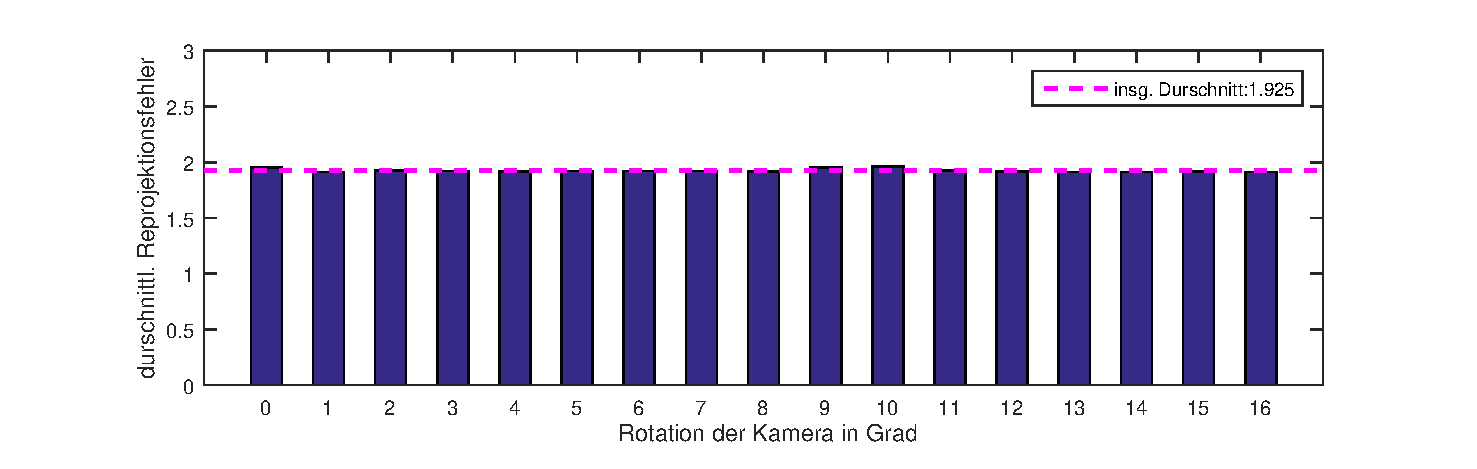
\includegraphics[width=\textwidth]{images/reprojectionErrorDeg2.eps}
	\caption{Einfluss der Rotation der Kamera}
	\label{fig:influenceRot}
\end{figure}


\section{Laufzeit der Entfaltung}
Durch den Kalibrierungsprozess erhalten wir zwei Abbildungsmatrizen (siehe Kapitel \ref{ch:implementation}), mit denen wir anschließend eine Reihe von Bildern entzerren möchten. Wir untersuchen dabei die Laufzeit pro gewählter Auflösung, in 50er Schritten, und ermitteln jeweils die Laufzeit gemittelt über 200 Bilder. Untersucht wird die Laufzeit bikubischer, sowie mit linearer Interpolation. 

\begin{figure}[!htb]
	\centering
	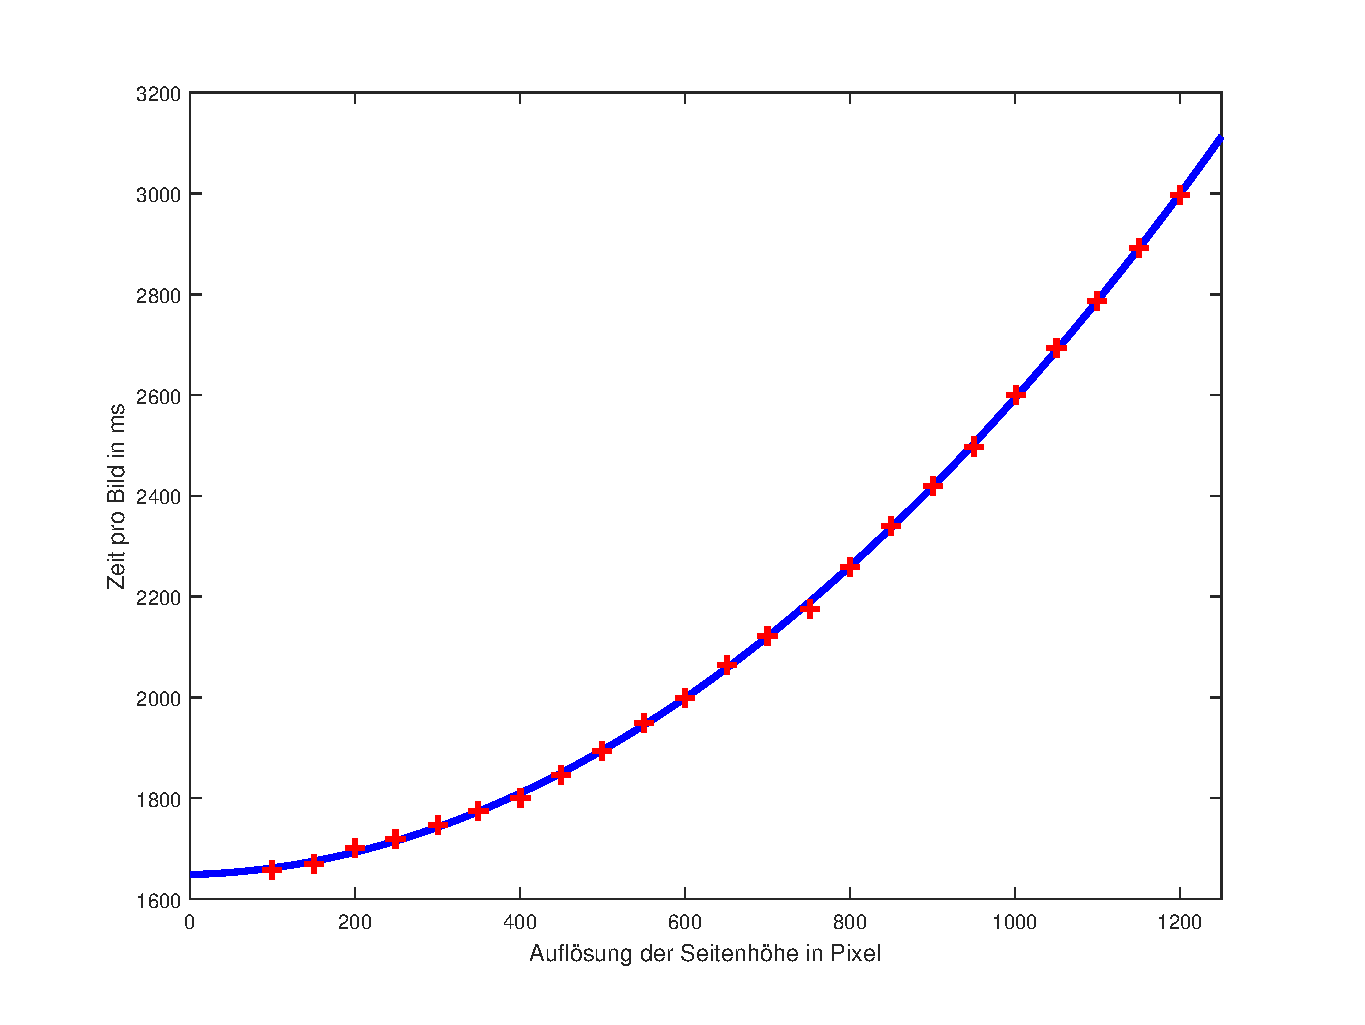
\includegraphics[width=0.8\textwidth]{images/runningTimePerSlantheight.eps}
	\caption{Einfluss der Ausgabeauflösung auf die Laufzeit der Entfaltung}
	\label{fig:influenceRes2}
\end{figure}



\section{Evaluierung des RANSAC zur Ellipsendetektion}
Die robuste Ellipsendetektion ist ein wichtiger Schritt bei der Entfaltung. Bei beiden Verfahren werden die bestimmten Ellipsen genutzt um Korrespondenzen zwischen den Sample-Positionen und Punkten auf dem Kegel im Weltkoordinatensystem herzustellen. Bei der Vorwärtsentfaltung werden die Ellipsen darüber hinaus benötigt, um für die Pixel geeignete 3D-Koordinaten interpolieren zu können. Es ist also von großer Bedeutung wie gut die Ellipsendetektion mittels RANSAC funktioniert.  


\begin{figure}[!htb]
	\centering
	\begin{subfigure}{.5\textwidth}
		\centering
		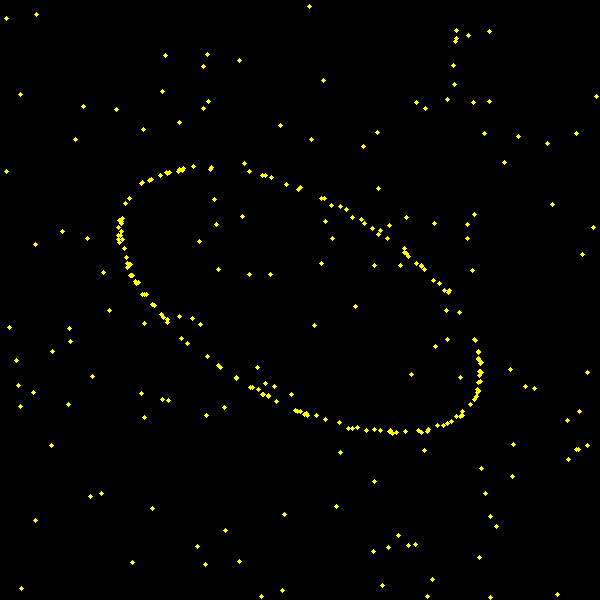
\includegraphics[width=.9\textwidth]{images/ransac50_0.png}
		\caption{gestörte Messdaten}
	\end{subfigure}%
	\begin{subfigure}{.5\textwidth}
		\centering
		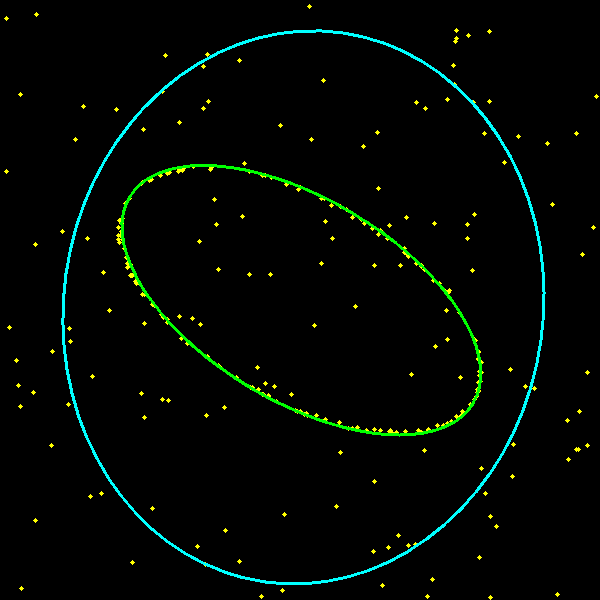
\includegraphics[width=.9\textwidth]{images/ransac50_1.png}
		\caption{detekt. Ellipsen: RANSAC (grün), LSQ (cyan)}
	\end{subfigure}
	\label{fig:bla}
	\caption{Vergleich RANSAC und LSQ bei gleichverteilten Ausreißern $\epsilon = 0.5, p = 0.99$}
\end{figure}

In unserem Verfahren ist eine Gleichverteilung der Ausreißer unwahrscheinlich. Viel wahrscheinlicher ist es, dass eine der nächst äußeren Ellipsen frühzeitig sichtbar wird (siehe Kapite \ref{s:ellipseDetection}). 

\begin{figure}[!htb]
	\begin{subfigure}{.5\textwidth}
		\centering
		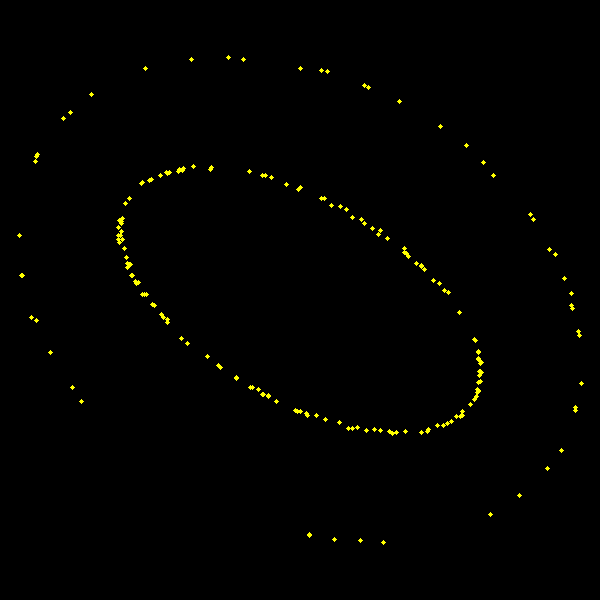
\includegraphics[width=.9\textwidth]{images/ransacShadow25_0.png}
	\end{subfigure}%
	\begin{subfigure}{.5\textwidth}
		\centering
		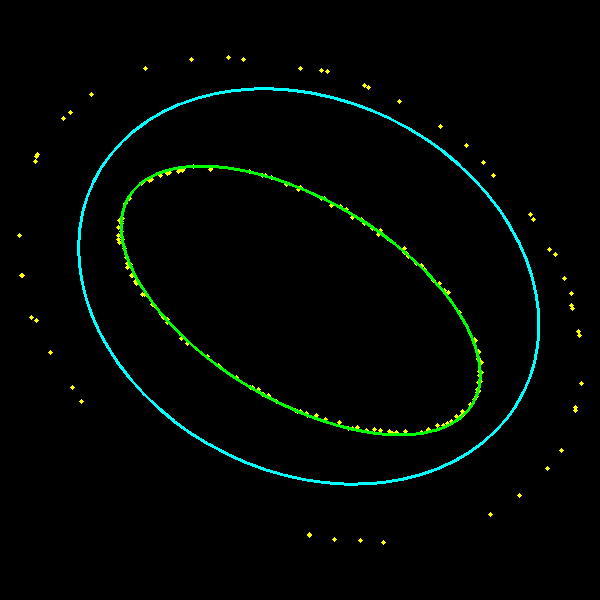
\includegraphics[width=.9\textwidth]{images/ransacShadow25_1.png}
	\end{subfigure}
	\begin{subfigure}{.5\textwidth}
		\centering
		\vspace{0.2cm}
		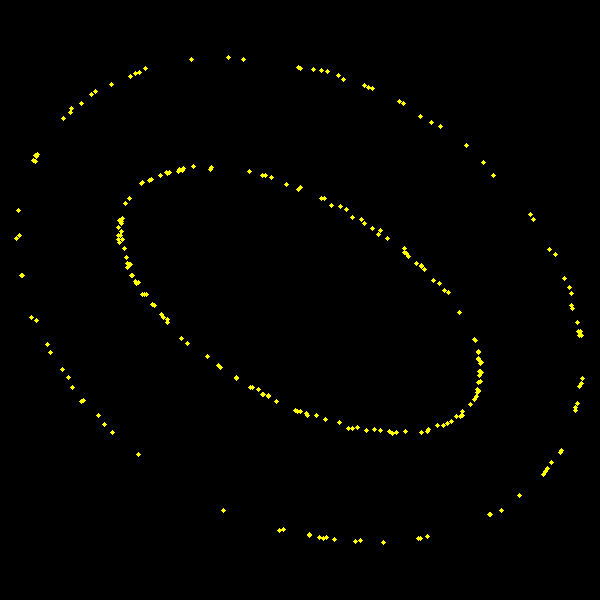
\includegraphics[width=.9\textwidth]{images/ransacShadow40_0.png}
	\end{subfigure}%
	\begin{subfigure}{.5\textwidth}
		\centering
		\vspace{0.2cm}
		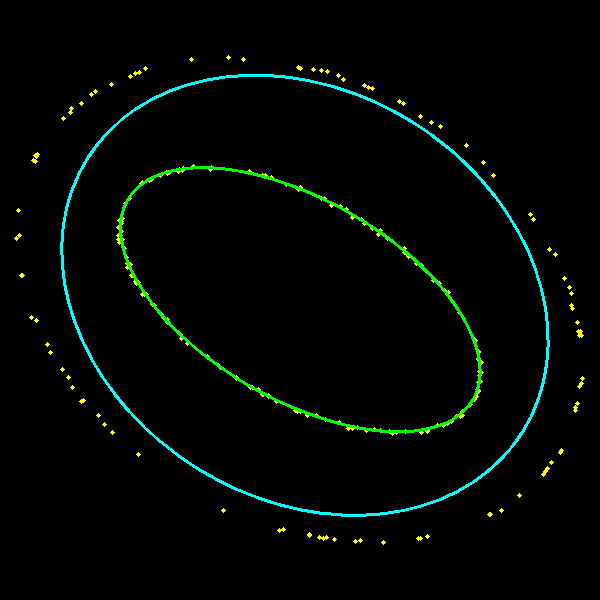
\includegraphics[width=.9\textwidth]{images/ransacShadow40_1.png}
	\end{subfigure}
	\caption{Vergleich RANSAC und LSQ bei Schattenellipsen mit $p = 0.99$ und $\epsilon = 0.25$ (oben), $\epsilon = 0.4$ unten, links gestörte Messdaten, rechts detektierte Ellipsen RANSAC (grün), LSQ (cyan)}
	\label{fig:blubb}
\end{figure}























